\FloatBarrier
\section{Numerical Simulations}
We will now consider the numerical application of the mobility problem for multiple swimmers and the use of the KIFFMM in solving the stokeslet element of the problem. 

\subsection{Rods in Shear flow}
In order to benchmark the use use of KIFMM in the case of mobility problems we propose to look at the problem of rods in a shear flow. We will consider prolate spheroid rods with minor axis of $0.15$ and a major axis of $1$ arranged in a triangular lattice with rod to rod spacing of $0.4$. In order to impose motion on the rods a shear flow is imposed on the fluid such that the rods want to locally rotate about the y axis. This is imposed through setting the fluid velocity of each force point on the swimming problem to be $\bm{u} = (\gamma\cdot x_3,0,0)$ where $\gamma$ denotes the magnitude of the shear flow and $x_3$ the z coordinate of the force points positions. We consider the two versions of the problem both with approximately the same number of quadrature points but with varying number of swimmers. The first problem involves 203 rods arranged in a triangular lattice of size $[5.2 \times 5.2]$ each discretised with 420 quadrature points for a total of 255780 SDOF. The second problem is 2016 rods discredited with 42 quadrature points for a total of 254,016 SDFOF.  For the KIFMM method we will use 500 particles in a node with 152 quadrature points as this provided a reasonably accurate approximation to the the vector product while still keeping computation times reasonable. A regularisation parameter of $\epsilon=1e-2$ was set to allow for regularisation error and a standard Nyström was implemented such that the performance of just the use of the KIFMM for Mobility problems considered. The use of NEAREST implementation can be considered later in the case of Squirmers. Due to the complexity of the fluid system with a large number of degrees of freedom and close boundaries we will also consider optimisation to the method which could help reduce the overall computation time of the problem in the hope of allowing for larger problem to be concidered in the future. 


\begin{figure}[!ht]
        \centering
        \begin{subfigure}[b]{0.475\textwidth}
            \centering
            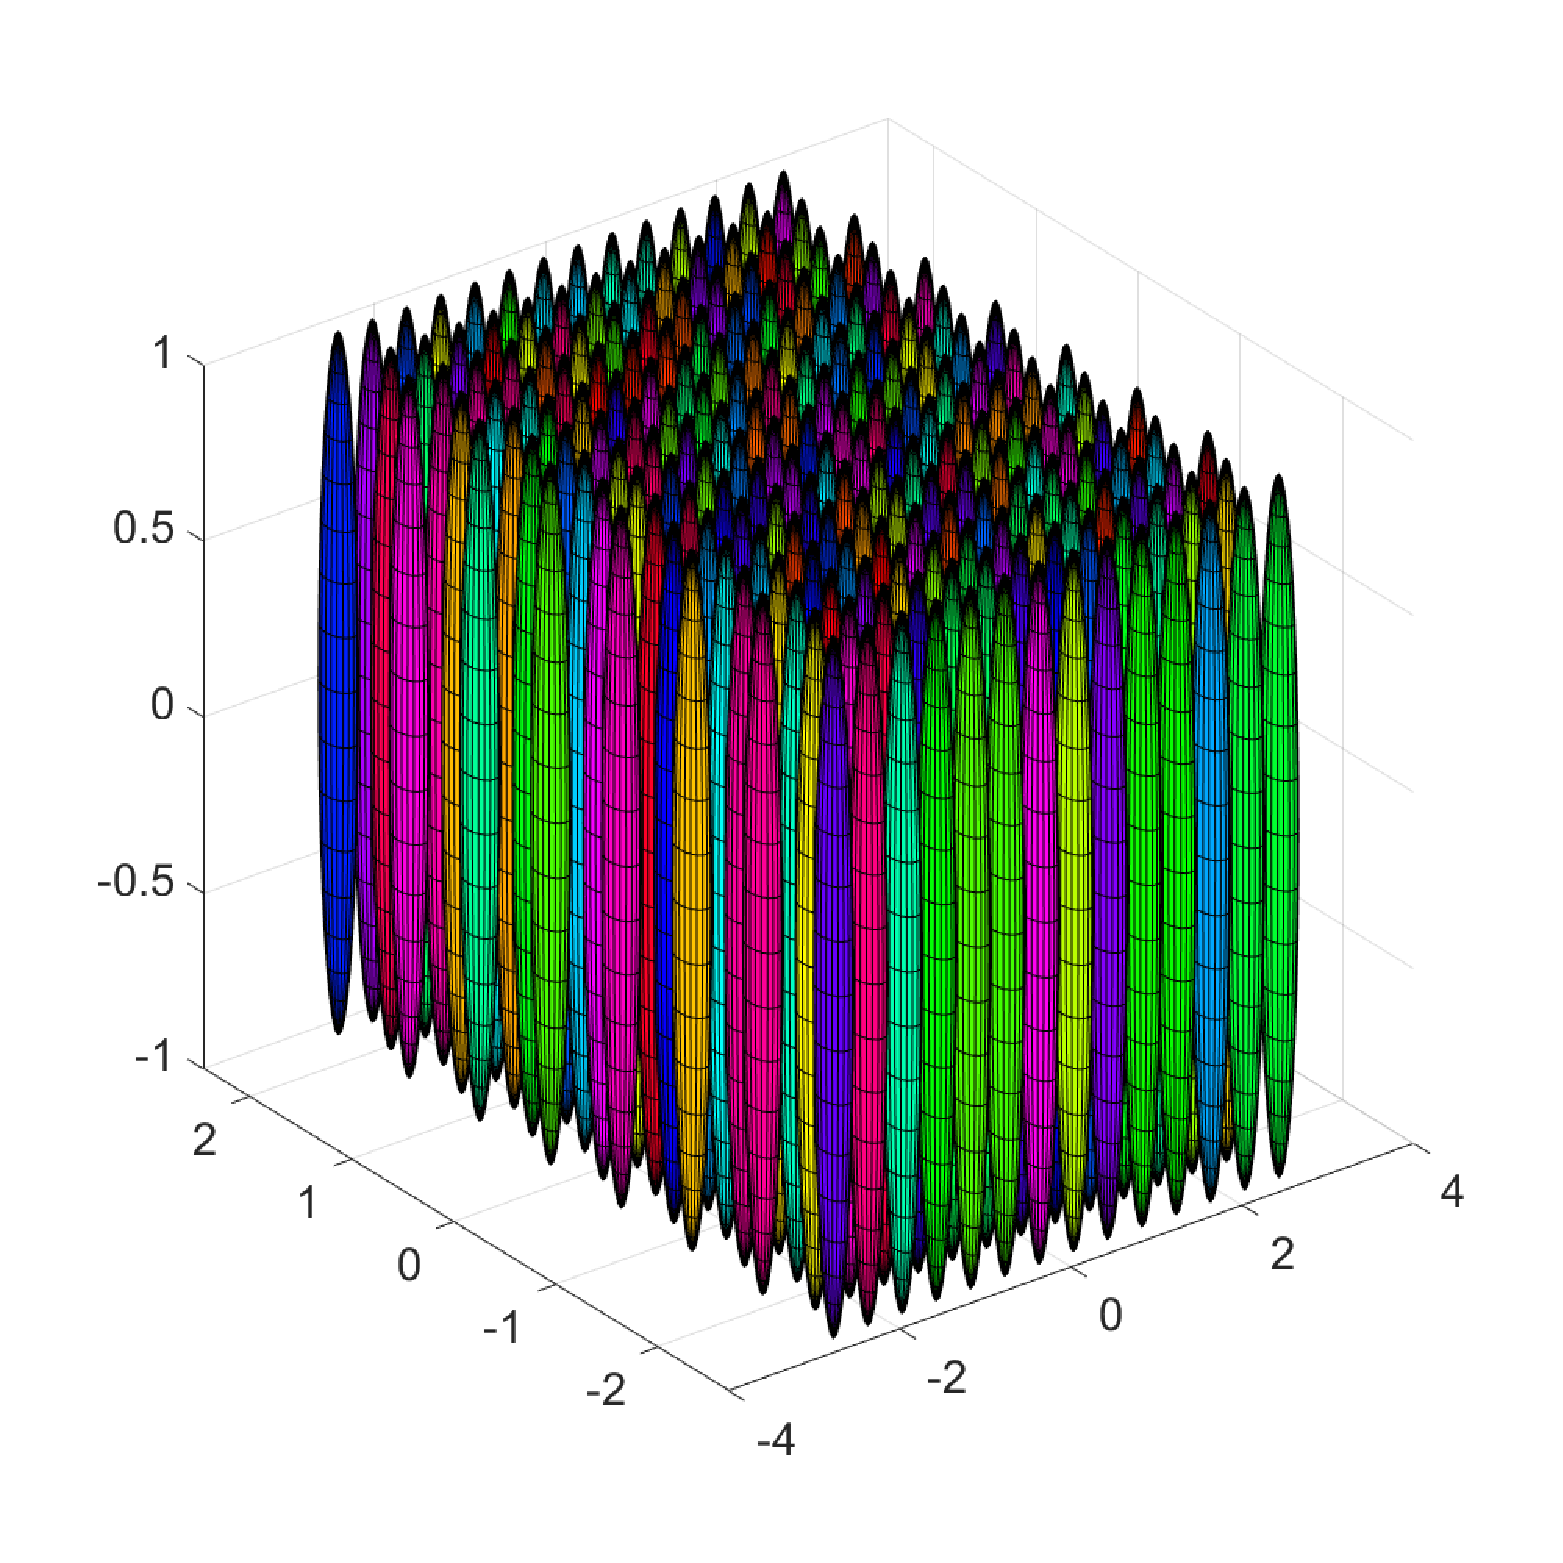
\includegraphics[width=\textwidth]{Images/Rods/SmallRods3d.pdf}
            \caption[]%
            {{\small 203 prolate spheroids in 3d View}}    
            \label{fig:mean and std of net14}
        \end{subfigure}
        \hfill
        \begin{subfigure}[b]{0.475\textwidth}  
            \centering 
            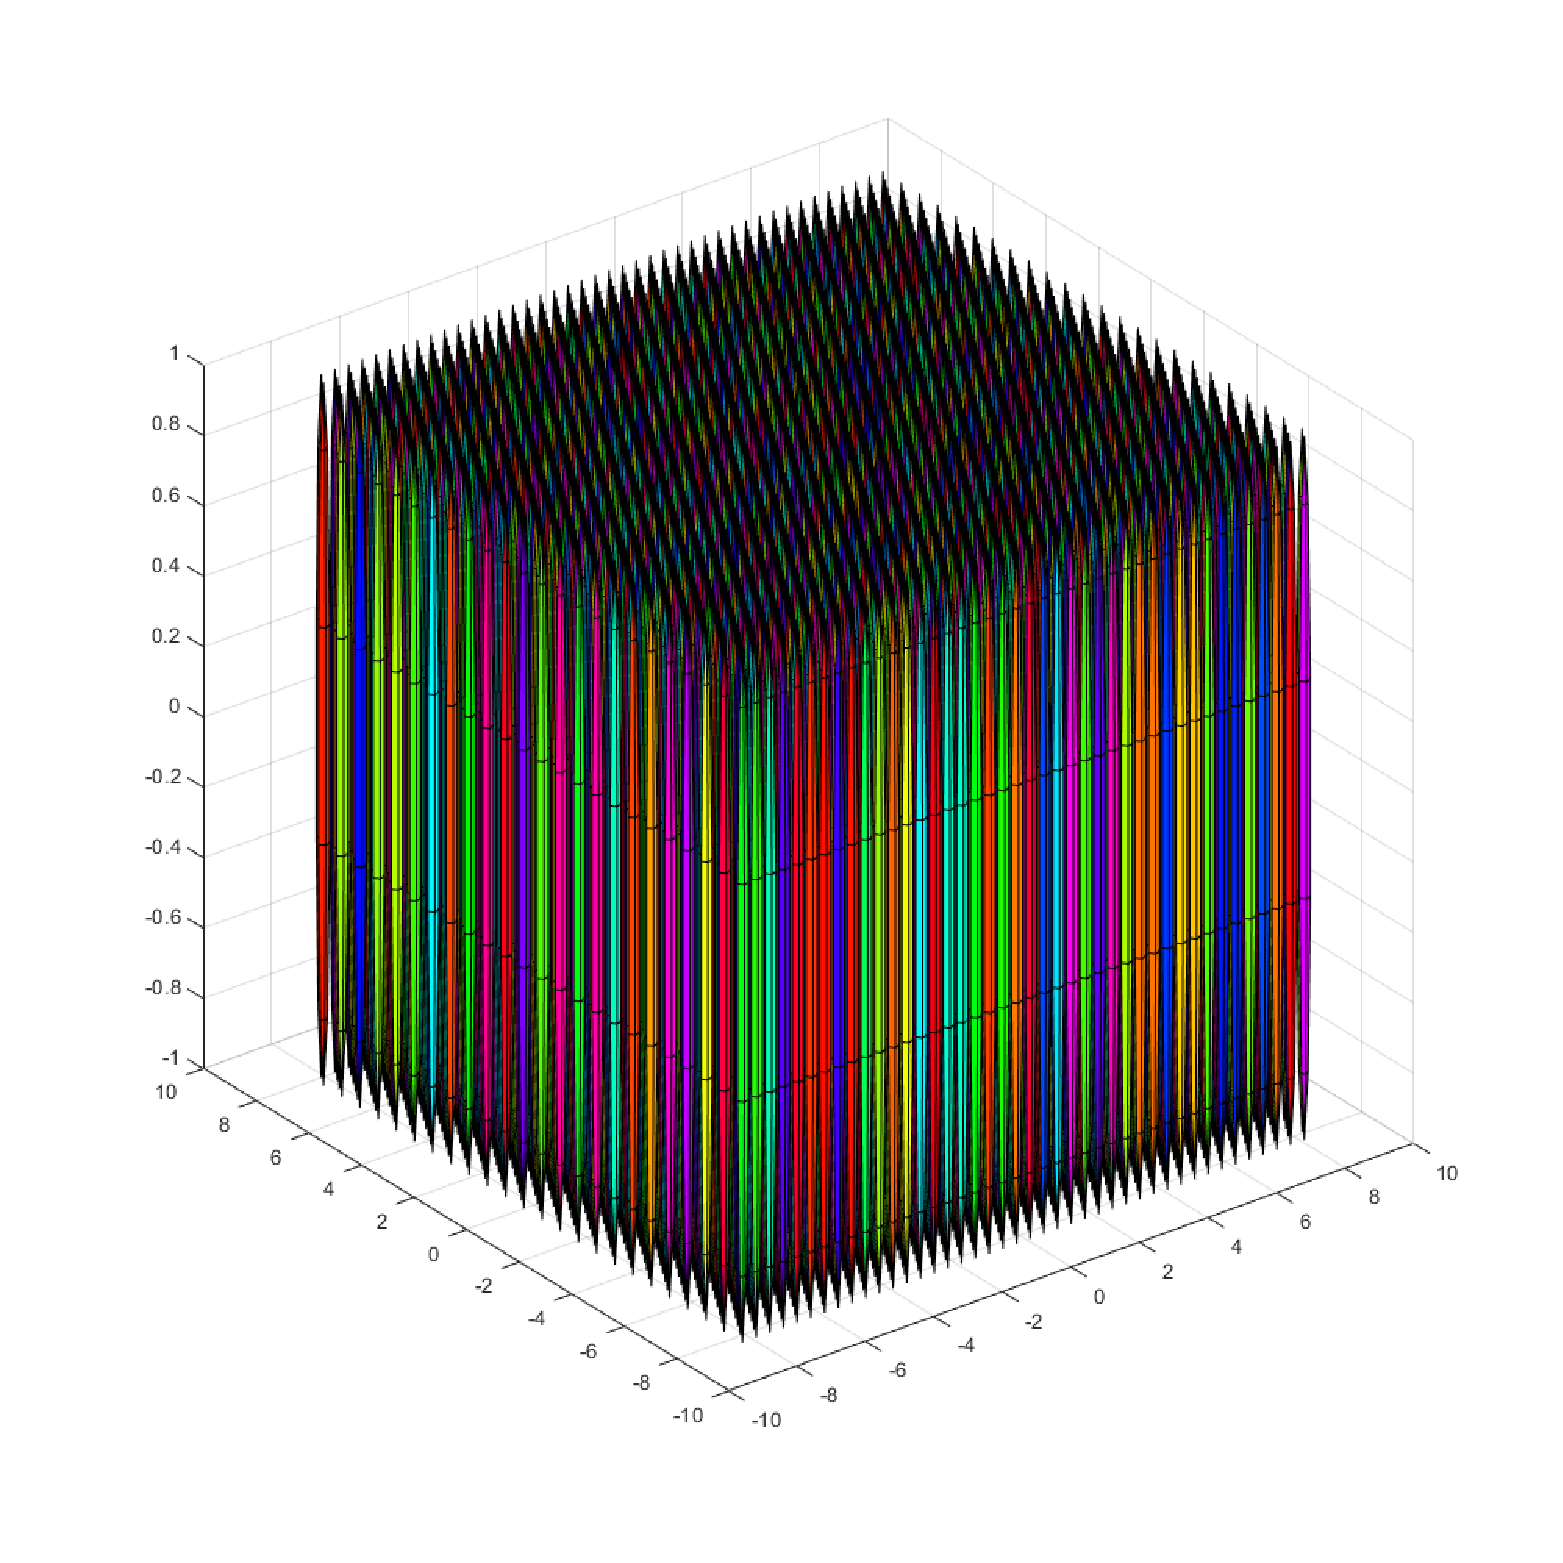
\includegraphics[width=\textwidth]{Images/Rods/LargeRods3d.pdf}
            \caption[]%
            {{\small 2016 prolate spheroids in 3d View}}    
            \label{fig:mean and std of net24}
        \end{subfigure}
        \vskip\baselineskip
        \begin{subfigure}[b]{0.475\textwidth}   
            \centering 
            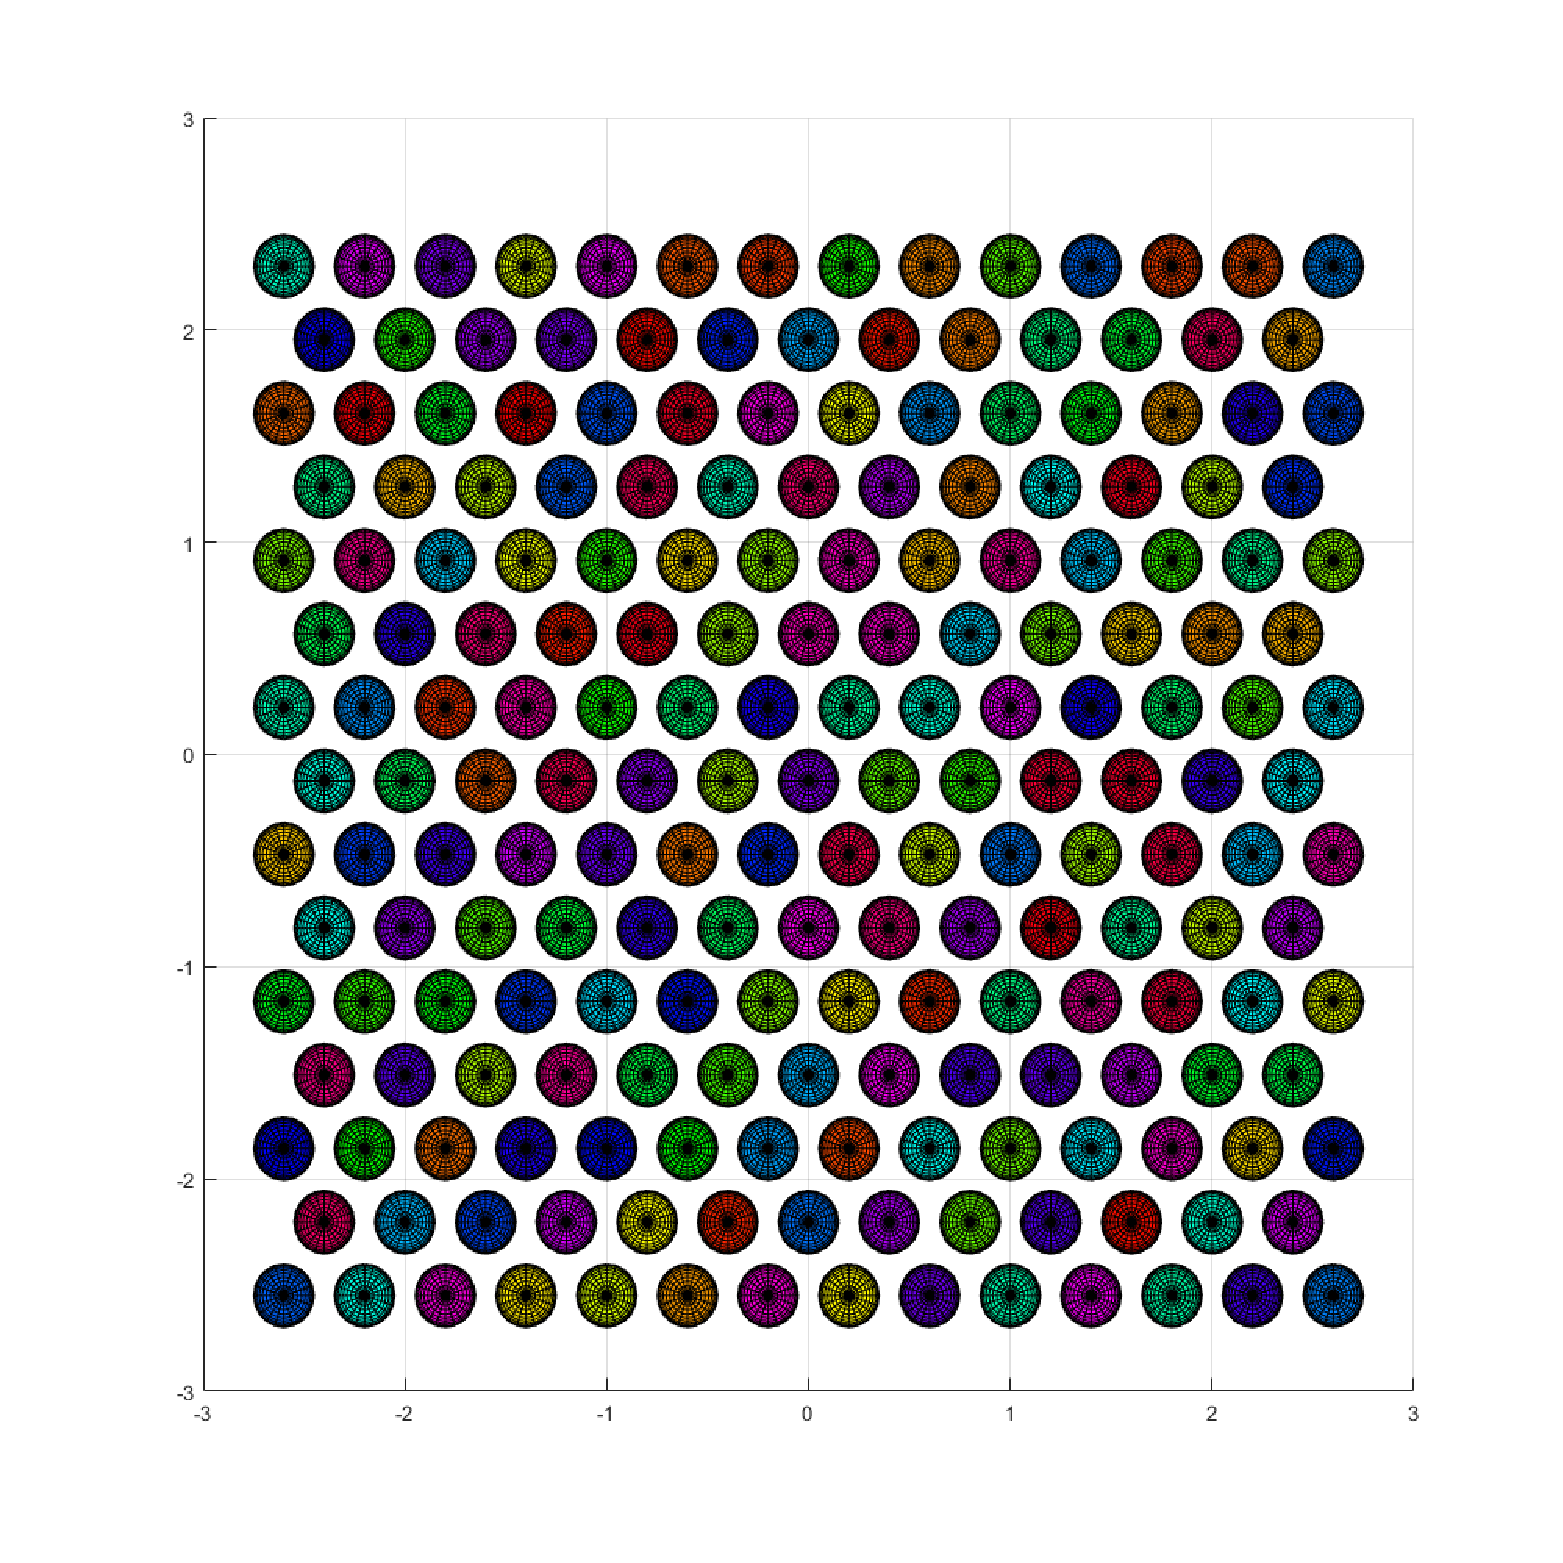
\includegraphics[width=\textwidth]{Images/Rods/SmallRodstop.pdf}
            \caption[]%
            {{\small 203 prolate spheroids from top down view}}    
            \label{fig:mean and std of net34}
        \end{subfigure}
        \hfill
        \begin{subfigure}[b]{0.475\textwidth}   
            \centering 
            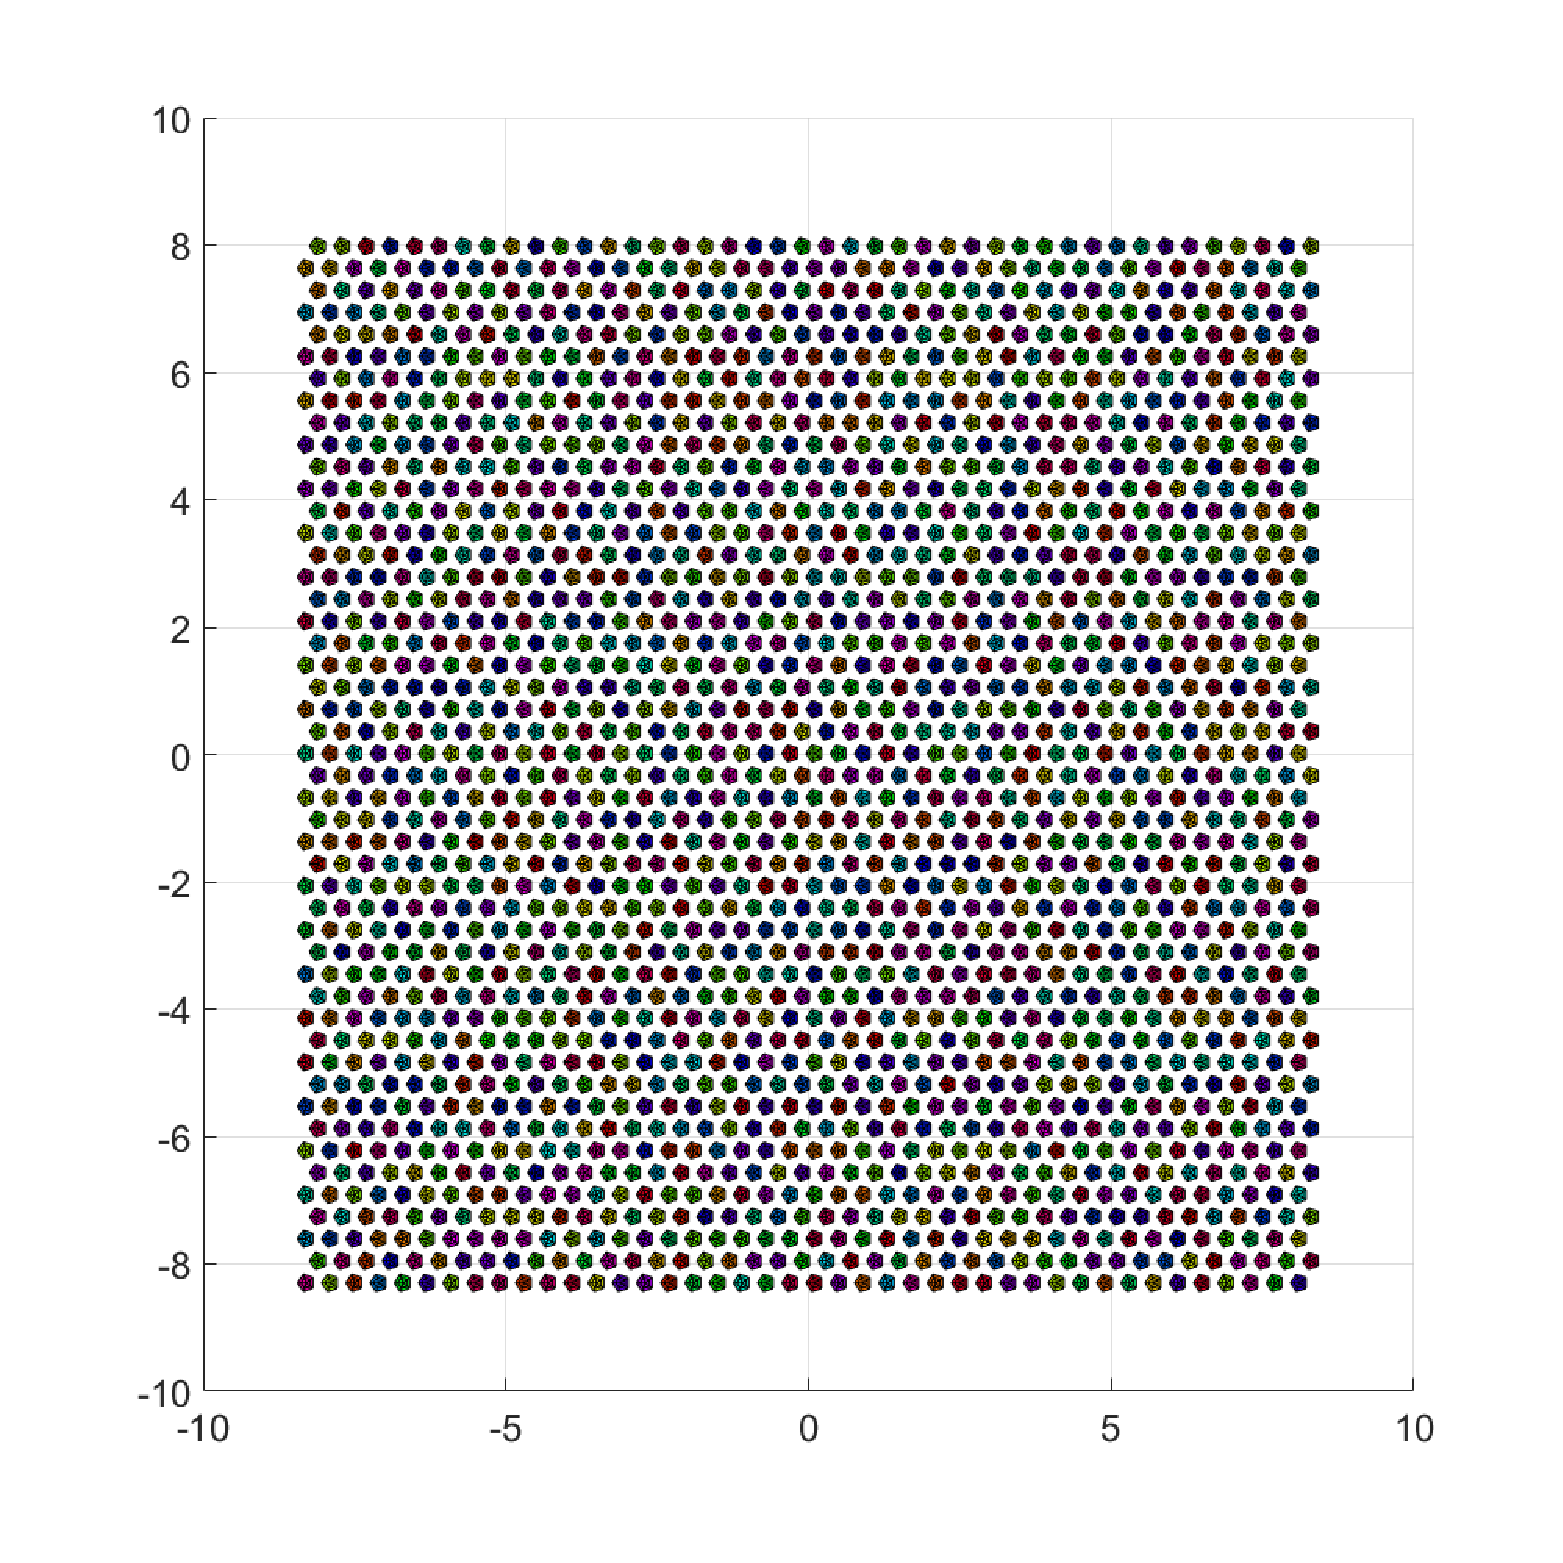
\includegraphics[width=\textwidth]{Images/Rods/LargeRodstop.pdf}
            \caption[]%
            {{\small 2016 prolate spheroids from top down view}}    
            \label{fig:mean and std of net44}
        \end{subfigure}
        \caption[Images of Rods in Shear flow]
        {\small Figure showing the configuration of prolate spheroids used in the two problems considered. Both problems are arranged on the same lattice spacing of $0.4$ units between each rod. A shear flow of 2 runs vertically from top to bottom such that the fluid velocity at the top has magnitude 1 at the top of the rods travelling in the positive x direction (Left to right) and magnitude 1 at the bottom of the rods travailing in the negative x direction (Right to left). This causes the rods to want to rotate about there central axis. } 
        \label{fig:mean and std of nets}
    \end{figure}


\subsection{Optimisations for the repeated evaluation of the KIFMM algorithm}
We will be solving this system through the use of GMRES (see \cref{appendix:GMRES}) as we are unable to form the full matrix with the KIFMM method. We can instead compute the matrix in block, we will compute the stokeslet matrix $A$ with the KIFMM method first before constructing the $B_i^U$, $B_i^\Omega$, $B_i^F$ and $B_i^M$ matrix blocks. For notational ease we will group these into two matrices
\begin{equation*}
\arraycolsep=0.4pt\def\arraystretch{1}
B = \left( \begin{array}{ccc}
B_{1}^{F} & B_{2}^{F} & B_{3}^{F} \\
B_{1}^{M} & B_{2}^{M} & B_{3}^{M}
\end{array}\right) \text{ and }
B^\prime = \left(\begin{array}{cc}
B_{1}^{U} & B_{1}^{\Omega} \\
B_{2}^{U} & B_{2}^{\Omega} \\
B_{3}^{U} & B_{3}^{\Omega} \\
\end{array}\right).
\end{equation*} 
We construct both $B$ and $B^\prime$ outside of the GMRES method as they remain the same, we could also consider doing this for the KIFMM method as our discretisation points remain fixed for all GMRES iterations and as such so do the stokeslet kernel matrices uses. This would speed up the method as the majority of the computation in the KIFMM method is in the generation of the stokeslet kernel, particularly for the multipole to multipole translation (\cref{eq:M2L}) and dense particle to particle interactions. This however would take a significant amount of memory as the stokeslet matrices needed for each M2L translation would need to be stored. A proposed optimisation is to use fast Fourier transforms to instead compute the M2L translation. Considering a M2L translation of the potential $\{\bm{f}^{AU}\}$ of a node $A$ onto the downwards surface $\{\bm{q}^{BD}\}$ of a node $B$. Both the upwards and downwards equivalent potentials are defined to be a Cartesian grid with the same number of quadrature points, by padding the centre of each surface with gridpoints of $0$ density we can view the M2L translation as a 3D convolution \cite{Ying2004} that can be carried out efficiently by FFT. We would only need to compute a single FFT and IFFT (inverse fast Fourier transform) per node and element wide multiplication for each node in the $V$ or $W$ interaction lists. We have yet to implement this method, but look to explore this approach if further research requires it.

In the hope to speed up the GMRES method without changing the underlying KIFMM method we will look at reducing the required number of GMRES iterations required to converge to the required tolerance.

\subsubsection{Initial Guess}\label{sec:Guess}

An easily implemented attempt at reducing the total number of GMRES iterations is to provide an initial guess to the GMRES solver such that the initial relative residual error is already minimised and the number of iterations required to converge will be lower. As seen in \cref{appendix:ConNum} the condition number of the system decreases and the eigenvalues more clustered with decreasing $\epsilon$, this means that in most cases the required number of GMRES iterations required for systems for the system to converge will be smaller as seen in \cref{fig:InitalGuessEPS}.
\begin{figure}[ht]
    \centering
    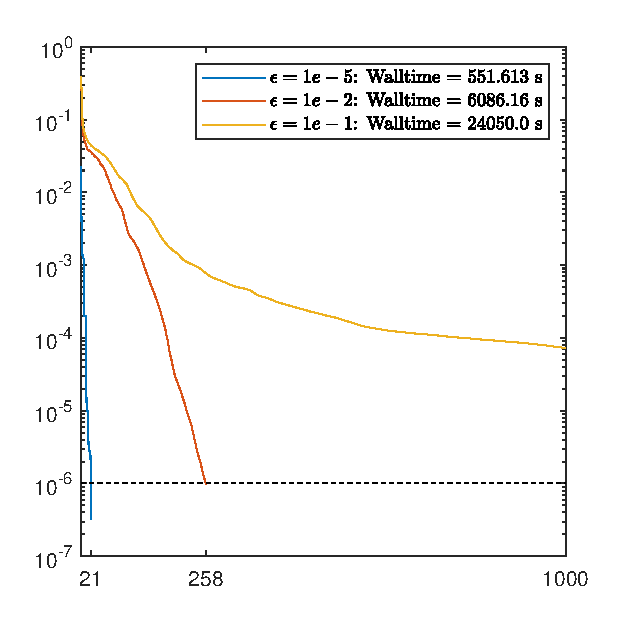
\includegraphics[width=0.5\textwidth]{Images/InitalGuessEPS.pdf}
    \caption{Convergence of the small rod problem with 3 different choices of epsilon. The $\epsilon = 1e-1$ problem did not converge in the given 1000 iterations.}
    \label{fig:InitalGuessEPS}
\end{figure}
Solving the problem for a smaller epsilon, however, does not give us an accurate initial guess for the actual problem with a larger epsilon as the particle interactions are of a smaller magnitude. However, we note that the stokeslet matrix $A$ is dominated by the diagonal elements whose magnitude is proportional to $1/\epsilon$. If we consider two versions of the problem one with a smaller value of epsilon $\epsilon_1$ and stokeslet matrix $A_1$ and a target epsilon $\epsilon_2$ with a stokeslet matrix $A_2$ for which we would like to solve the problem for. We first solve the initial problem with $\epsilon=\epsilon_1$, this should converge quickly in comparison to the second system and will return us a solution $\bm{F}_1$. The contribution to the first $3N_{F}$ terms are dominated by the diagonal elements of $\epsilon$ of order $1/\epsilon_1$ so by re-scaling the using a factor of $\epsilon_1/\epsilon_2$ we should have a better approximation to the solution. Very little has been published on the use of initial guesses with GMRES as often they provide little to no benefit to the overall computation. What is understood is the need for the residual from the initial guess $x_0$ need to be lower than the residual of the right-hand side $b$ ($\lVert b-Ax_0 \rVert \leq \lVert r_o \rVert$). In order to achieve this, we use a trick outlined by Heged{\"u}s \cite{Saad1986GMRES:Systems,Strakos2005OnComputations} which minimises the residual using the method of least squares to obtain a scaling factor of 
\begin{equation*}
    \left\|r_{0}\right\|=\left\|b-A_2 \bm{F}_1 \zeta_{\min }\right\|=\min _{\zeta}\left\|b-A_2 \bm{F}_1 \zeta\right\|, \quad \zeta_{\min }=\frac{b^{T} A_2 \bm{F}_1}{\left\|A_2 \bm{F}_1\right\|^{2}}
    \label{eq:Hegedus}
\end{equation*}
where $\bm{F}_1$ is our initial guess from $A_2$ and our initial guess for the GMRES algorithm is $x_0 = \zeta_{\min} \bm{F}_1$. This initial guess gave some improvement in both cases as seen in \cref{tab:Preconditioning}.

\subsubsection{Rescaling Mobility Matrix} \label{sec:Rescale}
In the hope of cheaply reducing the condition of the matrix and moretightly cluster the eigenvalues of the mobility matrix such that the GMRES algorithm converges in a smaller number of iterations \cite{CampbellGMRES}. We do this by rescaling the $B$ matrix in \cref{eq:mobilityStructure} such that its maximum value is one, This should reduce the of condition of the matrix and cluster the eigenvalues at the centre. We are able to do this due to the $0$ force and moment constrains we have imposed upon the system and as such we are able to rescale out $B$ matrix without affecting the constraints. 
We do see a tighter clustering in the eigenvalues shown in \cref{appendix:ConNum} where the eigenvalues cluster closer to 1, however the overall condition of the system increases.


\subsubsection{Preconditioning} \label{sec:Preconditioning}
A more optimal way in which we can solve Kyolov subspace methods is to use a preconditioner such that the matrix system we are trying to solve has a smaller condition number with more clustered eigenvalues. If we call the mobility matrix defined in \cref{eq:mobilityStructure} $M$, the vector of unknowns $\bm{x}$ and the right hand side $\bm{b}$ then we can refer to the system as $Mx=b$. The Matrix $M$ is much more badly conditioned (see \cref{appendix:ConNum}) than the stokeslet matrix $A$ as such requires a significant number of iterations to solve. Often when using problems GMRES we need to use a preconditioner to improve the condition number of the system we are solving, This reduced the effect of small perturbations made by the GMRES method.


Our preconditioner is based on work by Rostami and Olson \cite{Rostami2019FastBiofluids} and is inspired by the so-called “least-squares commutator” preconditioner \cite{Elman2005FiniteDynamics}. As described above we group the augmenting matrices into two larger matrices denoted $B$ and $B^\prime$. This means our mobility matrix can be written as 
\begin{equation*}
\begin{aligned}
\def\arraystretch{0.8}
    M = \left(\begin{array}{cc}
        A & B^\prime \\
        B & 0_{6N_{sw}\times6N_{sw}} 
    \end{array}\right) &= 
    \left(\begin{array}{cc}
        \mathds{1}_{3N_F \times 3N_F} & O_{3N_F\times6N_{sw}} \\
        BA^{-1} & \mathds{1}_{6N_{sw} \times 6N_{sw}}
    \end{array}\right)
    \left(\begin{array}{cc}
        A & B^\prime \\
        O_{6N_{sw}\times3N_F} & -BA^{-1}B^\prime
    \end{array}\right) \\
    &= LU.
\end{aligned}
\end{equation*}
This means $MU^{-1}$ has eigenvalues of 1 and as such GMRES should converge in one iterations \cite{Rostami2019FastBiofluids} if $U^{-1}$ is used as a right preconditioner to solve the system $MU^{-1}y = b$ where $x = U^{-1}y$. However due to the need to solve $BA^{-1}B^\prime$ this becomes infeasible particularly when we do not construct $A$ explicitly.  Instead, we will attempt to cheaply approximate $U^{-1}$, We will denote the preconditioner matrix 
\begin{equation}
\def\arraystretch{0.8}
    P_M = \left(\begin{array}{cc}
        P_A & B^\prime \\
        O_{6N_{sw}\times3N_F} & P_S
    \end{array}\right)
    \label{eq:Precon}
\end{equation}
where $P_A$ is a preconditioner for the matrix $A$ and $P_S$ is a preconditioner for $-BA^{-1}B^\prime$. Schurs complement \cite{Zhang2005TheApplications,Lu2002InversesMatrices} allows us to compute the inverse of a $2 \times 2$ block matrix as 
\begin{equation*}
\def\arraystretch{0.8}
    \left(\begin{array}{cc}
        A & B \\
        C & D
    \end{array}\right)^{-1} = \left(\begin{array}{cc}
A^{-1}+A^{-1} B\left(D-C A^{-1} B\right)^{-1} C A^{-1} & -A^{-1} B\left(D-C A^{-1} B\right)^{-1} \\
-\left(D-C A^{-1} B\right)^{-1} C A^{-1} & \left(D-C A^{-1} B\right)^{-1}
\end{array}\right) 
\end{equation*}
if $A$ is invertible. This gives that the inverse of our preconditioner matrix \cref{eq:Precon} is
\begin{equation*}
\def\arraystretch{0.8}
        P_M^{-1} = \left(\begin{array}{cc}
        P_A^{-1} & -P_A^{-1} B^T P_S^{-1} \\
        O_{6N_{sw}\times3N_F} & P_S^{-1}
    \end{array}\right)
\end{equation*}
We, therefore, need to solve two systems of equations involving $P_A$ and one linear system involving $P_S$. As we stated above solving a linear system involving $P_S$ is too computationally challenging to form and solve so we must look for an approximation to this solution. Inspired by the method of least square we look for a solution $C$ which minimises the residual of $\lVert AB^T - B^\prime C \rVert \;\forall\; C \in \mathbb{R}^{6N_{sw}\times6N_{sw}}$. This solutions is found by taking the square of the residual to obtain $(AB^T - B^\prime C)^T(AB^T - B^\prime C) = (AB^T)^T(AB^T)-(AB^T)^TB^\prime C-C^T(B^\prime)^TA^T + C^T(B^\prime)^TB^\prime C$. Taking the derivative of this with respect to $C$ equal to $0$ will minimise the residual squared. This gives us that $-2(B^\prime)^TAB^T + 2(B^\prime)^TB^\prime C=0$ so $C = ((B^\prime)^TB^\prime)^{-1}(B^\prime)^TAB^T$. Computing the inverse of $C$ we get that $C^{-1} = ((B^\prime)^TAB^T)^{-1}((B^\prime)^TB^\prime)$. As we have minimised the residual we can say that $AB^T \approx B^\prime C \implies B^T C^{-1} = A^{-1}B^\prime$. Substituting both of these into our equation for our preconditioner $P_S$ gives us that, 
\begin{equation}
\begin{aligned}
    P_S = - B A^{-1}B^\prime &= -B B^{T} C^{-1} \\
    & = -(B B^{T})((B^\prime)^TAB^T)^{-1}((B^\prime)^TB^\prime) \\
    \implies P_S^{-1} &= -((B^\prime)^TB^\prime)^{-1}((B^\prime)^TAB^T)(B B^{T})^{-1}
\end{aligned}
\label{eq:PreconS}
\end{equation}
This means the computation of $P_S^{-1}$ now only involves solving the linear systems $(B^\prime)^TB^\prime$ and $B B^{T}$ however these are cheap and easy to solve as both matrices are mainly sparse with dominant diagonal elements due to their construction. We still need to compute the solution to $P_A^{-1}$. We will consider solving this we a block diagonal form of the KIFMM where we only consider the interactions between nodes. This captures most of the dominant interactions between particles and provides a relatively accurate estimation of the solution to $A^{-1}$ being significantly quicker to run. It also reduces the system to a smaller set of smaller problems, one for each node. These are quicker and easier for GMRES to solve and as such the method can converge quicker for these systems. This principle could be extended to include all nodes in the $U$ interaction list, this provides better results for a single pass however due to the off-diagonal elements now included the problem is worse conditioned with longer interactions times so we will only consider the purely block-diagonal preconditioner. Block diagonal preconditions have been used to solve problems in systems using the Rotne-Prager-Yamakawa (RPY) tensor \cite{UsabiagaHYDRODYNAMICSAPPROACH}, Stokeslet\cite{Nazockdast2017AMechanics} and more general elliptical PDEs \cite{Ibeid2018FastEquations}. Following on from using the diagonal preconditioner for $P_A^{-1}$ we will also consider a cheaper approximation to full matrix multiplication of $A$ in the computation of $P_S^{-1}$. Following on from the results shown in \cref{fig:QuadPoints} we note an accurate cheaper computation can be achieved by using fewer quadrature points for the equivalent surfaces, in particular 60 quadrature points was chosen as it provided as descent balance between the accuracy of the method and provides a noticeable speed up compared to the full method with 152 quadrature points. 

\subsection{Data}
The results of all 3 optimisations can be seen in \cref{tab:Preconditioning} along with data for the non preconditioned system. All method had a fixed stopping criterion of $\lVert Mx-b \rVert_2/\lVert b \rVert_2 \leq 1e-6$. The 2016 swimmer model proved challenging to solve with over 150 more GMRES iterations needed to solve the problem. Both method were aided by the use of an inital guess with the computation time of both being reduced by nearly 10\% as the inital iterations are replaced by quicker iterations using a smaller $\epsilon$ value. The attempt at rescaling the lower augmented matrix proved to increase the overall computation time where the tighter clustered eigenvalues did not allow the method to converge quicker as the maximum and minimum eigenvalues separated more leading to a worse conditioned system overall. When we precondition the system we see a dramatic decrease in computation time, particularly with the 2016 swimmer case where the computation time drops by 80\%. The 203 swimmer case does not see as much of a significant drop, possible due to the larger contribution the stokeslet matrix $A$ has. This being the hardest part to precondition will determine the overall effectiveness of our preconditioner. We would expect to see that for systems with more swimmers and the same number of quadrature points the number of GMRES to converge to stay approximately the same and as such larger system to be able to be tackled. Combinations of these methods may prove useful in reducing the calculation further such as inital guesses for preconditioned systems however due to the rapid decrease in the residual from the preconditioned system it is doubt full it will provide any noticeable gain and the need to use the Heged{\"u}s trick involves another full matrix product, It might prove more useful in solving the reduced system inside the the preconditioner where the number of iterations can be quite large and the system is more dominated by the diagonal elements. A better way to reduce the computation time would be to improved the GMRES method though recycling the Krylov subspaces in order to solve repetitive linear systems \cite{Parks2006RecyclingSystems,Rostami2019FastBiofluids}. When solving the precondition we need to solve $P_A^{-1}$ twice for each iteration. The equivalent matrix for each solve remains constant with only the right-hand side changing. Instead of forming the Krylov subspace from scratch we can use some vectors from an existing Krylov subspace and construct a new Krylov subspace based on them for the new right hand side. Reducing the overall number of iterations needed for subsequent solves. This would also help with calculating the grand resistance matrix \cref{eq:GrandResistance} where multiple solutions need to be found for different right hand sides.

\begin{table}[htbp]
\begin{singlespace}
\centering
\setlength{\tabcolsep}{6pt}
\renewcommand{\arraystretch}{1.4}
\small
\begin{tabular}{p{2cm} p{1cm} p{2cm} p{1.5cm} p{0.1cm} p{1cm} p{2cm} p{1.5cm}}
\multirow{2}{*}{\parbox{1.8cm}{number of swimmers}} & \multicolumn{3}{l}{No precondtioner} & & \multicolumn{3}{l}{Initial Guess} \\ \cline{2-4} \cline{6-8}
  & \# of iters & \# of MVPs ($M$) & walltime (sec.) & & \# of iters & \# of MVPs ($M_{\epsilon_1}/M_{\epsilon_2}$) & walltime (sec.) \\ \hline
  203 & 250 & 250 & 8599 & &  268 & 20/248 & 7763\\
  2016 & 409 & 409 & 23645 & & 358 & 12/346 & 20977\\ \hline
  \multirow{2}{*}{\parbox{1.8cm}{number of swimmers}} & \multicolumn{3}{l}{Rescaling} & &\multicolumn{3}{l}{Least-squares commutator} \\ \cline{2-4} \cline{6-8}
  & \# of iters & \# of MVPs ($M$) & walltime (sec.) & & \# of iters & \# of MVPs ($M/P_A^{-1}/A_S$) & walltime (sec.) \\ \hline
  203 & 297 & 297 & 9357 & & 71 & 64/130/65 & 6834 \\
  2016 & 523 & 523 & 34036 & & 47 & 47/96/48 & 4887 
\end{tabular}
\label{tab:Preconditioning}
\caption{Comparison of preconditioners in the case of Rods in Shear Flow. All methods converged to a tolerance of $1e-6$}
\end{singlespace}
\end{table}

\subsection{Squirmers}
